\documentclass[11pt,a4paper]{article}
\usepackage[margin=2.5cm]{geometry}
\usepackage{graphicx}
\usepackage{float}

\title{Report 4: Threads}
\author{Le Nguyen Minh Quang -- 2540093}
\date{\today}

\begin{document}
\maketitle

\section{Goal}
In labwork 3 I used \textbf{1D blocks}: the image was flattened into a
long list of pixels, and each thread took one pixel from that list. In
this labwork I change the grayscale kernel to use \textbf{2D blocks},
so the threads follow the shape of the image (rows and columns). Then I
try different 2D block sizes and compare the speed with the 1D version.

Like before, I ran the code on Google Colab with a \textbf{Tesla T4}
GPU. The test image is the same leaf photo as labwork 3,
$549 \times 364$ pixels (199\,836 pixels in total).

\section{Method}
\begin{itemize}
  \item \textbf{No flatten:} the image keeps its shape $(364, 549, 3)$
  and is copied to the GPU directly.
  \item \textbf{2D thread index:} each thread computes its column
  \texttt{tidx} and its row \texttt{tidy}:
  \begin{center}
    tidx = threadIdx.x + blockIdx.x $\times$ blockDim.x \\
    tidy = threadIdx.y + blockIdx.y $\times$ blockDim.y
  \end{center}
  \item \textbf{2D grid:} the block size is now a tuple, for example
  $(16, 16)$, and the grid size is also a tuple:
  \begin{center}
    gridSize = ($\lceil$ width / 16 $\rceil$,
                $\lceil$ height / 16 $\rceil$) = (35, 23)
  \end{center}
  \item \textbf{Boundary check:} $549$ and $364$ are not multiples of
  16, so some blocks on the right and bottom edges go outside the image.
  Those threads must do nothing, so I check both \texttt{tidx} and
  \texttt{tidy}.
  \item \textbf{Why \texttt{tidx} is the column:} threads next to each
  other in a warp have \texttt{threadIdx.x} next to each other. If
  \texttt{tidx} is the column, they read pixels that are next to each
  other in memory, which is faster (coalesced access).
  \item \textbf{Timing:} I used \texttt{time.time()} and ran each kernel
  once before measuring, because the first call also compiles it.
\end{itemize}

\section{Code}
\begin{verbatim}
@cuda.jit
def grayscale_2d(src, dst):
    tidx = cuda.threadIdx.x + cuda.blockIdx.x * cuda.blockDim.x
    tidy = cuda.threadIdx.y + cuda.blockIdx.y * cuda.blockDim.y
    if tidy < src.shape[0] and tidx < src.shape[1]:
        r = src[tidy, tidx, 0]
        g = src[tidy, tidx, 1]
        b = src[tidy, tidx, 2]
        gray = np.uint8((r + g + b) / 3)
        dst[tidy, tidx, 0] = gray
        dst[tidy, tidx, 1] = gray
        dst[tidy, tidx, 2] = gray

blockSize = (16, 16)
gridSize = (math.ceil(imageWidth / 16), math.ceil(imageHeight / 16))

devInput = cuda.to_device(inputImage)
devOutput = cuda.device_array((imageHeight, imageWidth, 3), np.uint8)
grayscale_2d[gridSize, blockSize](devInput, devOutput)
gpuOutput = devOutput.copy_to_host()
\end{verbatim}
Compared to labwork 3, the only changes are: a second index
\texttt{tidy}, a check on both directions, and tuples for
\texttt{blockSize} and \texttt{gridSize}.

\section{Results}

\subsection{CPU vs GPU (256 threads per block)}
For a fair comparison I used 256 threads per block in both versions:
256 for 1D and $16 \times 16$ for 2D. The GPU times include copying the
image to the GPU and back.

\begin{center}
\begin{tabular}{|l|r|r|}
\hline
                       & Time (ms) & Speedup \\ \hline
CPU                    & 784.81    & 1       \\ \hline
GPU 1D (256)           & 1.97      & 397     \\ \hline
GPU 2D ($16 \times 16$) & 1.44      & 545     \\ \hline
\end{tabular}
\end{center}
The 2D result is exactly the same as the CPU result
(\texttt{np.array\_equal} returns \texttt{True}).

Note: the CPU time is higher than in labwork 3 (256 ms) because this
time I loop over rows and columns of the 3D array, which is slower in
Python. The difference between 1D and 2D here comes mostly from the
copy time, which changes a bit from one run to another, so the next
test measures only the kernel.

\begin{figure}[H]
  \centering
  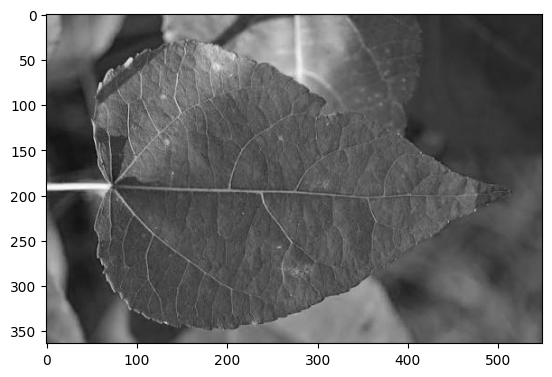
\includegraphics[width=0.6\textwidth]{gray_gpu_2d.png}
  \caption{Gray image from the 2D kernel.}
\end{figure}

\subsection{Block size vs speedup, 1D vs 2D}
Here the image is already on the GPU and I only measure the kernel. One
call is very short, so I ran each kernel 50 times and took the average.
Speedup = CPU time / kernel time.

\begin{center}
\begin{tabular}{|c|r|r|r|r|r|}
\hline
2D block & Threads & \multicolumn{2}{c|}{1D} & \multicolumn{2}{c|}{2D} \\
         & per block & Time (ms) & Speedup & Time (ms) & Speedup \\ \hline
$4 \times 4$   & 16   & 0.110 & 7\,143  & 0.105 & 7\,500  \\ \hline
$8 \times 8$   & 64   & 0.059 & 13\,229 & 0.055 & 14\,378 \\ \hline
$16 \times 16$ & 256  & 0.054 & 14\,577 & 0.056 & 14\,059 \\ \hline
$32 \times 32$ & 1024 & 0.057 & 13\,872 & 0.062 & 12\,569 \\ \hline
\end{tabular}
\end{center}

\begin{figure}[H]
  \centering
  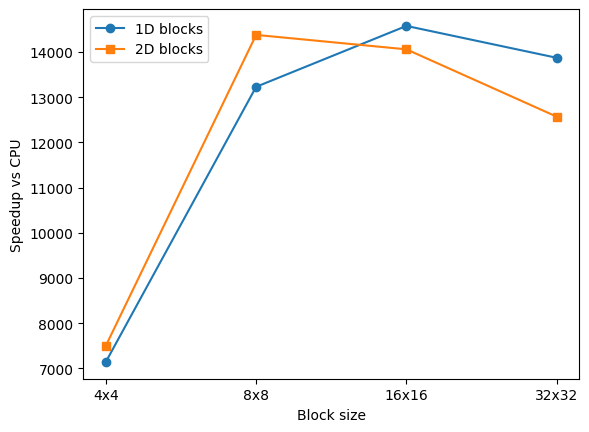
\includegraphics[width=0.7\textwidth]{blocksize_vs_speedup.png}
  \caption{Speedup vs block size, 1D and 2D blocks.}
\end{figure}

\section{Discussion}
\begin{itemize}
  \item \textbf{$4 \times 4$ is the slowest} (about 2$\times$ slower)
  for both 1D and 2D. A block of 16 threads fills only half of a warp
  (32 threads), so half of the GPU work is wasted. This is the same
  thing I saw in labwork 3.
  \item \textbf{From $8 \times 8$ up, the speed is almost the same}
  (about 0.055--0.062 ms). The best 2D block was $8 \times 8$, and the
  best 1D block was 256.
  \item \textbf{$32 \times 32$ in 2D is a little slower.} The grid must
  cover the whole image, so it covers $576 \times 384$ pixels instead
  of $549 \times 364$. About 10\% of the threads are outside the image
  and do nothing. With $8 \times 8$ blocks only about 2\% are wasted.
  \item \textbf{1D vs 2D:} the difference is less than 10\%, so for
  grayscale 2D blocks are not really faster. Grayscale works on each
  pixel alone, so the GPU does the same work in both cases. The real
  benefit of 2D blocks is that the code uses (row, column) directly,
  like the image. This will be useful for the next labworks (like
  blur), where a pixel needs its neighbours above and below.
\end{itemize}

\section{Exercises}

\subsection*{Exercise 1}
GPU limits: 512 threads/block, 1024 threads/SM, 8 blocks/SM.
\begin{itemize}
  \item $8 \times 8 = 64$ threads/block. Max 8 blocks/SM, so
  $8 \times 64 = 512$ threads/SM. Only half of the SM is used.
  \item $16 \times 16 = 256$ threads/block. $1024 / 256 = 4$ blocks/SM
  ($\le 8$), so $1024$ threads/SM. The SM is full.
  \item $32 \times 32 = 1024$ threads/block. This is more than 512
  threads/block, so it cannot be launched.
\end{itemize}
\textbf{Answer: $16 \times 16$.}

\subsection*{Exercise 2}
SM limits: 1536 threads, 4 blocks.
\begin{center}
\begin{tabular}{|r|r|r|}
\hline
Threads/block & Blocks in SM & Threads in SM \\ \hline
128  & 4 (block limit)           & 512  \\ \hline
256  & 4 (block limit)           & 1024 \\ \hline
512  & 3 ($3 \times 512 = 1536$)  & \textbf{1536} \\ \hline
1024 & 1 (2 would be 2048)       & 1024 \\ \hline
\end{tabular}
\end{center}
\textbf{Answer: 512 threads/block}, because it fills the SM completely.

\subsection*{Exercise 3}
Vector length 2000, block size 512. The number of blocks is
$\lceil 2000 / 512 \rceil = 4$, so the grid has
$4 \times 512 = $ \textbf{2048 threads}. The last 48 threads do nothing
(they fail the \texttt{if tid < n} check).

\section{Conclusion}
I changed the grayscale kernel from 1D to 2D blocks. The result is the
same as the CPU, and the GPU is about 14\,000$\times$ faster than the
CPU (kernel only). 1D and 2D blocks have almost the same speed for
grayscale. The block should have at least 32 threads (one warp), and
blocks like $8 \times 8$ or $16 \times 16$ are a good choice.

\end{document}
